% !TEX root = ./../../../_Thesis.tex

\begin{figure*}[!t]
	\centering

	\begin{tabular}{@{}r@{ } c@{ } c@{ } c@{ } c@{ } c }
%	&
%	\small{N} &
%	\small{C} &
%	\small{K} &
%	\small{Z} &
%	\small{O} & \\

	\begin{sideways} \parbox[b]{20mm} {Camera} \end{sideways} &
	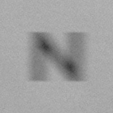
\includegraphics[width=0.185\textwidth]{__Images/05/WB_20-200_-2@90/wb_N_20-200_Camera-2,00D@90(lens).png} &
	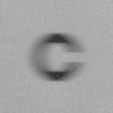
\includegraphics[width=0.185\textwidth]{__Images/05/WB_20-200_-2@90/wb_C_20-200_Camera-2,00D@90(lens).png} &
	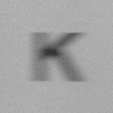
\includegraphics[width=0.185\textwidth]{__Images/05/WB_20-200_-2@90/wb_K_20-200_Camera-2,00D@90(lens).png} &
	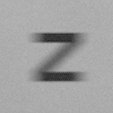
\includegraphics[width=0.185\textwidth]{__Images/05/WB_20-200_-2@90/wb_Z_20-200_Camera-2,00D@90(lens).png} &
	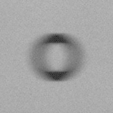
\includegraphics[width=0.185\textwidth]{__Images/05/WB_20-200_-2@90/wb_O_20-200_Camera-2,00D@90(lens).png} \\

	\begin{sideways} \parbox[b]{20mm} {Simulation} \end{sideways} &
	
\includegraphics[width=0.185\textwidth]{__Images/05/WB_20-200_-2@90/wb_N_20-200_Camera-2,00D@90(simulated).png} &
	
\includegraphics[width=0.185\textwidth]{__Images/05/WB_20-200_-2@90/wb_C_20-200_Camera-2,00D@90(simulated).png} &
	
\includegraphics[width=0.185\textwidth]{__Images/05/WB_20-200_-2@90/wb_K_20-200_Camera-2,00D@90(simulated).png} &
	
\includegraphics[width=0.185\textwidth]{__Images/05/WB_20-200_-2@90/wb_Z_20-200_Camera-2,00D@90(simulated).png} &
	
\includegraphics[width=0.185\textwidth]{__Images/05/WB_20-200_-2@90/wb_O_20-200_Camera-2,00D@90(simulated).png} \\

	\begin{sideways} \parbox[b]{20mm} {Local~SSIM} \end{sideways} &
	
\includegraphics[width=0.185\textwidth]{__Images/05/WB_20-200_-2@90/wb_N_20-200_Camera-2,00D@90(comparison).png} &
	
\includegraphics[width=0.185\textwidth]{__Images/05/WB_20-200_-2@90/wb_C_20-200_Camera-2,00D@90(comparison).png} &
	
\includegraphics[width=0.185\textwidth]{__Images/05/WB_20-200_-2@90/wb_K_20-200_Camera-2,00D@90(comparison).png} &
	
\includegraphics[width=0.185\textwidth]{__Images/05/WB_20-200_-2@90/wb_Z_20-200_Camera-2,00D@90(comparison).png} &
	
\includegraphics[width=0.185\textwidth]{__Images/05/WB_20-200_-2@90/wb_O_20-200_Camera-2,00D@90(comparison).png} \\

	\begin{sideways} \parbox[b]{20mm} {Difference} \end{sideways} &
	
\includegraphics[width=0.185\textwidth]{__Images/05/WB_20-200_-2@90/wb_N_20-200_Camera-2,00D@90(diff).png} &
	
\includegraphics[width=0.185\textwidth]{__Images/05/WB_20-200_-2@90/wb_C_20-200_Camera-2,00D@90(diff).png} &
	
\includegraphics[width=0.185\textwidth]{__Images/05/WB_20-200_-2@90/wb_K_20-200_Camera-2,00D@90(diff).png} &
	
\includegraphics[width=0.185\textwidth]{__Images/05/WB_20-200_-2@90/wb_Z_20-200_Camera-2,00D@90(diff).png} &
	
\includegraphics[width=0.185\textwidth]{__Images/05/WB_20-200_-2@90/wb_O_20-200_Camera-2,00D@90(diff).png} \\

	\end{tabular}
	
	\caption[Comparisons of our simulated results against ground truth obtained with a astigmatic camera]{Comparisons of our simulated results against ground truth obtained with a astigmatic camera. These large images correspond to a Snellen ratio of 20/200. (top row) Images captured using the DSLR camera with an extra cylindrical lens with -2 diopters at the vertical meridian. (second row) Our simulated results. (third row) SSIM metric results. (fourth row) AD metric.}
	\label{fig:comparison_astig-2@90_wb}
\end{figure*}
